\documentclass[tikz, border=5mm, 12pt]{standalone}
\usepackage{amsmath}
\usepackage{amsfonts}

\usetikzlibrary{arrows.meta,shadows,positioning,calc,decorations.markings}

\pgfdeclarelayer{timelines}
\pgfsetlayers{timelines,main}

\begin{document}

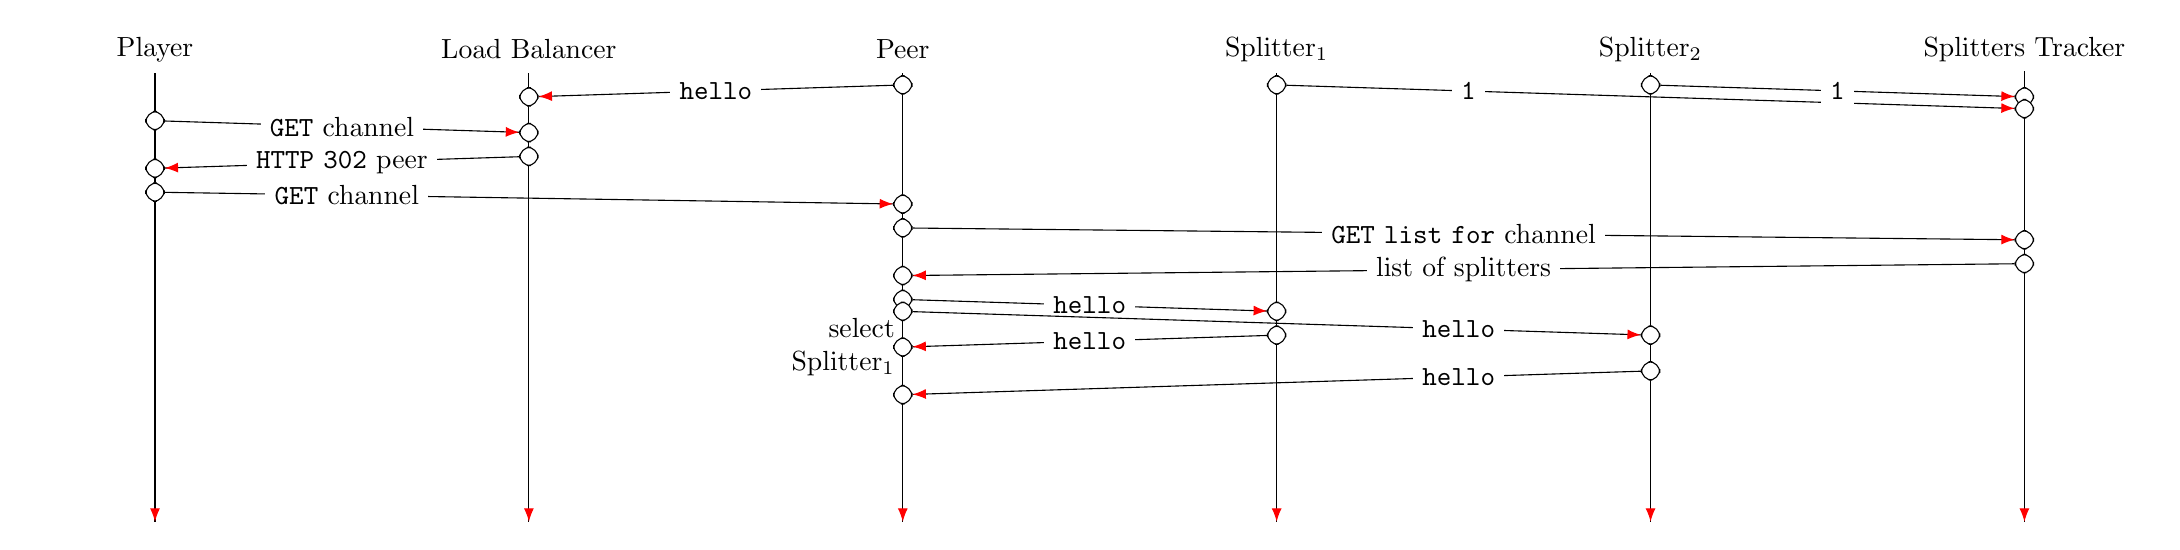
\begin{tikzpicture}
  
  \tikzset{myptr/.style={decoration={markings,mark=at position 1 with %
        {\arrow[red,scale=1.0,>=Latex]{>}}},postaction={decorate}}}
  
  % Entities
  \node[] (Player) {\parbox{3cm}{\centering Player}};
  \node[right=1.5 of Player] (Balancer) {\parbox{3cm}{\centering Load Balancer}};
  \node[right=1.5 of Balancer] (Peer) {\parbox{3cm}{\centering Peer}};
  \node[right=1.5 of Peer] (Splitter1) {\parbox{3cm}{\centering Splitter$_1$}};
  \node[right=1.5 of Splitter1] (Splitter2) {\parbox{3cm}{\centering Splitter$_2$}};
  \node[right=1.5 of Splitter2] (Tracker) {\parbox{3cm}{\centering Splitters Tracker}};

  % Timelines
  \begin{pgfonlayer}{timelines}
    \coordinate (Pla) at ($(Player.center) + (0.0,-6)$);
    \draw[myptr] ($(Player.center) + (0,-2ex)$) -- (Pla);  
    \coordinate (Bal) at ($(Balancer.center) + (0.0,-6)$);
    \draw[myptr] ($(Balancer.center) + (0,-2ex)$) -- (Bal);
    \coordinate (Pee) at ($(Peer.center) + (0.0,-6)$);
    \draw[myptr] ($(Peer.center) + (0,-2ex)$) -- (Pee);
    \coordinate (Sp1) at ($(Splitter1.center) + (0.0,-6)$);
    \draw[myptr] ($(Splitter1.center) + (0,-2ex)$) -- (Sp1);
    \coordinate (Sp2) at ($(Splitter2.center) + (0.0,-6)$);
    \draw[myptr] ($(Splitter2.center) + (0,-2ex)$) -- (Sp2);
    \coordinate (Tra) at ($(Tracker.center) + (0.0,-6)$);
    \draw[myptr] (Tracker) -- (Tra);
  \end{pgfonlayer}
  % Time steps
  
  % 00
  \node (00) at ($(Player) + (-2ex,-3ex)$) {};
  \node (Pe00) at ($(Peer) + (0,-3ex)$) [fill=white!100,draw,rounded corners] {};
  \node (Ba00) at ($(Balancer) + (0,-4ex)$) [fill=white!100,draw,rounded corners] {};
  \node (S100) at ($(Splitter1) + (0,-3ex)$) [fill=white!100,draw,rounded corners] {};
  \node (S200) at ($(Splitter2) + (0,-3ex)$) [fill=white!100,draw,rounded corners] {};
  \node (Tr001) at ($(Tracker) + (0,-4ex)$) [fill=white!100,draw,rounded corners] {};
  \node (Tr002) at ($(Tracker) + (0,-5ex)$) [fill=white!100,draw,rounded corners] {};
  \draw[myptr] (Pe00) -- (Ba00) node [pos=0.5,fill=white!100] {$\mathtt{hello}$};
  \draw[myptr] (S100) -- (Tr002) node [pos=0.25,fill=white!100] {$\mathtt{1}$};
  \draw[myptr] (S200) -- (Tr001) node [pos=0.5,fill=white!100] {$\mathtt{1}$};
  
  % 01
  \node (01) at ($(00) + (0,-3ex)$) {};
  \path let \p{Player}=(Player),\p{01}=(01) in node (Pl01) at (\x{Player},\y{01}) [fill=white!100,draw,rounded corners] {};
  \node (011) at ($(00) + (0,-4ex)$) {};
  \path let \p{Balancer}=(Balancer),\p{011}=(011) in node (Ba01) at (\x{Balancer},\y{011}) [fill=white!100,draw,rounded corners] {};
  \draw[myptr] (Pl01) -- (Ba01) node [pos=0.5,fill=white!100] {$\mathtt{GET}~\text{channel}$};

  % 02
  \node (02) at ($(01) + (0,-3ex)$) {};
  \path let \p{Balancer}=(Balancer),\p{02}=(02) in node (Ba02) at (\x{Balancer},\y{02}) [fill=white!100,draw,rounded corners] {};
  \node (021) at ($(01) + (0,-4ex)$) {};
  \path let \p{Player}=(Player),\p{021}=(021) in node (Pl02) at (\x{Player},\y{021}) [fill=white!100,draw,rounded corners] {};
  \draw[myptr] (Ba02) -- (Pl02) node [pos=0.5,fill=white!100] {$\mathtt{HTTP~302}~\text{peer}$};

  % 03
  \node (03) at ($(02) + (0, -3ex)$) {};
  \path let \p{Player}=(Player),\p{03}=(03) in node (Pl03) at (\x{Player},\y{03}) [fill=white!100,draw,rounded corners] {};
  \node (031) at ($(02) + (0,-4ex)$) {};
  \path let \p{Peer}=(Peer),\p{031}=(031) in node (Pe03) at (\x{Peer},\y{031}) [fill=white!100,draw,rounded corners] {};
  \draw[myptr] (Pl03) -- (Pe03) node [pos=0.25,fill=white!100] {$\mathtt{GET}~\text{channel}$};

  % 04
  \node (04) at ($(03) + (0, -3ex)$) {};
  \path let \p{Peer}=(Peer),\p{04}=(04) in node (Pe04) at (\x{Peer},\y{04}) [fill=white!100,draw,rounded corners] {};
  \node (041) at ($(03) + (0,-4ex)$) {};
  \path let \p{Tracker}=(Tracker),\p{041}=(041) in node (Tr04) at (\x{Tracker},\y{041}) [fill=white!100,draw,rounded corners] {};
  \draw[myptr] (Pe04) -- (Tr04) node [pos=0.5,fill=white!100] {$\mathtt{GET~list~for}~\text{channel}$};

  % 05
  \node (05) at ($(04) + (0, -3ex)$) {};
  \path let \p{Tracker}=(Tracker),\p{05}=(05) in node (Tr05) at (\x{Tracker},\y{05}) [fill=white!100,draw,rounded corners] {};
  \node (051) at ($(04) + (0,-4ex)$) {};
  \path let \p{Peer}=(Peer),\p{051}=(051) in node (Pe05) at (\x{Peer},\y{051}) [fill=white!100,draw,rounded corners] {};
  \draw[myptr] (Tr05) -- (Pe05) node [pos=0.5,fill=white!100] {$\text{list~of~splitters}$};

  % 06
  \node (06) at ($(05) + (0, -3ex)$) {};
  \path let \p{Peer}=(Peer),\p{06}=(06) in node (Pe06) at (\x{Peer},\y{06}) [fill=white!100,draw,rounded corners] {};
  \node (061) at ($(05) + (0,-4ex)$) {};
  \path let \p{Peer}=(Peer),\p{061}=(061) in node (Pe061) at (\x{Peer},\y{061}) [fill=white!100,draw,rounded corners] {};
  \node (062) at ($(05) + (0,-6ex)$) {};
  \path let \p{Splitter1}=(Splitter1),\p{061}=(061) in node (S106) at (\x{Splitter1},\y{061}) [fill=white!100,draw,rounded corners] {};
  \draw[myptr] (Pe06) -- (S106) node [pos=0.5,fill=white!100] {$\mathtt{hello}$};
  \path let \p{Splitter2}=(Splitter2),\p{062}=(062) in node (S206) at (\x{Splitter2},\y{062}) [fill=white!100,draw,rounded corners] {};
  \draw[myptr] (Pe061) -- (S206) node [pos=0.75,fill=white!100] {$\mathtt{hello}$};

  % 07
  \node (07) at ($(06) + (0, -3ex)$) {};
  \path let \p{Splitter1}=(Splitter1),\p{07}=(07) in node (S107) at (\x{Splitter1},\y{07}) [fill=white!100,draw,rounded corners] {};
  \node (071) at ($(06) + (0,-4ex)$) {};
  \path let \p{Peer}=(Peer),\p{071}=(071) in node (Pe071) at (\x{Peer},\y{071}) [fill=white!100,draw,rounded corners] {};
  \node (072) at ($(06) + (0,-6ex)$) {};
  \node (073) at ($(06) + (0,-8ex)$) {};
  \path let \p{Peer}=(Peer),\p{073}=(073) in node (Pe073) at (\x{Peer},\y{073}) [fill=white!100,draw,rounded corners] {};
  \draw[myptr] (S107) -- (Pe071) node [pos=0.5,fill=white!100] {$\mathtt{hello}$};
  \path let \p{Splitter2}=(Splitter2),\p{072}=(072) in node (S207) at (\x{Splitter2},\y{072}) [fill=white!100,draw,rounded corners] {};
  \draw[myptr] (S207) -- (Pe073) node [pos=0.25,fill=white!100] {$\mathtt{hello}$};
  \node (Sel) at ($(Pe071) + (-5ex,0)$) {\begin{tabular}{r} select \\ Splitter$_1$ \end{tabular}};
  
\end{tikzpicture}
\end{document}
